\documentclass[11pt]{article}
\usepackage[cm]{fullpage}
%%AVC PACKAGES
\usepackage{avcgreek}
\usepackage{avcfonts}
\usepackage{avcmath}
\usepackage[numberby=section]{avcthm} % 
\usepackage{qcmacros}
\usepackage{goldstone}
%%MACROS FOR THIS DOCUMENT
\numberwithin{equation}{section}
\usepackage[
  margin=1.5cm,
  includefoot,
  footskip=30pt,
  headsep=0.2cm,headheight=1.3cm
]{geometry}
\usepackage{fancyhdr}
\pagestyle{fancy}
\fancyhf{}
\fancyhead[LE,RO]{Quiz 1, Handout 1: Hartree-Fock Equations}
\fancyfoot[CE,CO]{\thepage}
\usepackage{url}

\begin{document}

\section{Hartree-Fock Theory}

The goal of electronic structure theory is to solve the ``clamped-nuclei'' Schr\"odinger equation
\begin{align}
\label{eq:electronic-schrodinger-equation}
	\op{H}\Y_k
=&\
	E_k\Y_k
&
  \op{H}
=&\
  V_{\mr{nuc}}
+
	\op{H}_e
=
  \sum_{a<b}^{\text{nuc.}}
	\fr{Z_aZ_b}{|\bo{R}_a-\bo{R}_b|}
-
  \fr{1}{2}
  \sum_i^{\text{elec.}}
	\nabla_i^2
-
  \sum_a^{\text{nuc.}}
  \sum_i^{\text{elec.}}
	\fr{Z_a}{|\bo{R}_a-\bo{r}_i|}
+
  \sum_{i<j}^{\text{elec.}}
	\fr{1}{|\bo{r}_i-\bo{r}_j|}
\end{align}
with an optimal balance of accuracy and efficiency for the problem of interest.
The most accurate solution possible for a given atomic orbital (AO) basis set\footnote{cc-pVXZ, 6-31G, ANO1, etc.} results from expanding the wavefunction
\begin{align}
\label{eq:full-ci-wavefunction-expansion}
	\Y_k
=&\
	\sum_\mu
	\F_\mu c_{\mu k}
\end{align}
in terms of all possible Slater determinants ($n$-electron basis functions $\{\F_\mu\}$) that can be formed from an orthonormal one-electron basis of spin-orbitals, $\{\y_p\}$.
The expansion coefficients $(\bo{c})_k=c_{\mu k}$ are eigenvectors of the matrix $(\bo{H})_{\mu\nu}=\ip{\F_\mu|\op{H}|\F_\nu}$, which is the matrix representation of the Hamiltonian in the determinant basis.
This is called the {\it full configuration-interaction} (FCI) solution.

Any one-electron basis spans the same ``function space'' as the AO basis set itself, and the full $n$-electron basis $\{\F_\mu\}$ spans the same space of $n$-electron functions regardless of how one forms spin orbitals from the AO basis set.
As a result, one obtains the same FCI solution for any choice of spin-orbitals.
In general, however, FCI solutions are completely unfeasible for basis sets of sufficient size to approach the complete basis set limit.
One can think of this as a simple counting problem: if there are $m$ functions in the AO basis, then there are $2m$ spin-orbitals in the one-electron basis,\footnote{$m$ $\a$-orbitals and $m$ $\b$-orbitals.} and there are ``$2m$ choose $n$'' \footnote{The number of unique sets of $n$ marbles that can be drawn from a bag of $2m$ marbles.  See \url{http://en.wikipedia.org/wiki/Combination}}
\begin{align*}
{2m \choose n}\equiv\fr{(2m)!}{n!(2m-n)!}
\end{align*}
unique Slater determinants in the $n$-electron basis that can be formed from the spin MOs.
The upshot is that we usually have to omit some Slater determinants in order get an answer in a reasonable amount of time.

As soon as we truncate our determinant expansion (\ref{eq:full-ci-wavefunction-expansion}), our choice of spin MOs makes a significant difference in the quality of our results.
In particular, we need to choose our set of one-electron functions to minimize the number of Slater determinants it takes to ``get close to'' the exact wavefunction.


\subsection{Defining the problem}

It can be shown that optimizing $\ip{\Y|\op{H}_e|\Y}$ by varying $\Y$ subject to the normalization constraint $\ip{\Y|\Y}=1$ is equivalent to solving the Schr\"odinger equation.
When we further constrain the form of $\Y$ this is no longer true, but it \textit{does} generally allow us to get the best approximation to $\Y$ for a given approach (or ``Ansatz'').

In order to make the wavefunction expansion converge with a relatively small number of $\F_\mu$s, we wish to find the best single-determinant approximation to $\Y$.
That is, we wish to optimize
\begin{align}
	\ip{\F|\op{H}_e|\F}
\sp\sp
	\F(1,\ld,n)
=
\fr{1}{\sqrt{n!}}
\left|\ar{
	\y_1(1)&\y_2(1)&\cd&\y_n(1)\\
	\y_1(2)&\y_2(2)&\cd&\y_n(2)\\
	\vd    &\vd    &\dd&\vd    \\
	\y_1(n)&\y_2(n)&\cd&\y_n(n)}\right|
\end{align}
with respect to variation of the orbitals $\{\y_p\}$, enforcing the normalization constraint by keeping the spin orbitals orthonormal.
Note that here the function argument $(i)$ is shorthand for $(\bo{r}_i,s_i)$ where $\bo{r}_i$ denotes the position of the $i\eth$ electron and $s_i$ denotes its spin.
This optimization problem is the essence of \textit{Hartree-Fock theory}.

Once we have solved for the Hartree-Fock optimization problem, the expectation value $\ip{\F|\op{H}_e|\F}$ is itself a good first approximation to the electronic energy.
More importantly, however, when we use this new set of Hartree-Fock spin-orbitals, $\{\y_p\}$, the FCI expansion tends to converge much more quickly to the true wavefunction.
Specifically, when we rewrite equation~\ref{eq:full-ci-wavefunction-expansion} in terms of single $\{\F_i^a\}$, double $\{\F_{ij}^{ab}\}$, triple $\{\F_{ijk}^{abc}\}$, etc.\ replacements \footnote{It is typical to use dummy indices $i,j,k,l$ to count over the orbitals in the reference determinant $\F$ -- the ``occupied orbitals'' -- and to use $a,b,c,d,$ to count over the orbitals not contained in $\F$ -- the ``unoccupied'' or ``virtual orbitals.''  Dummy indices $p,q,r,s$ are generally used to count over the full set of spin-orbitals, whether occupied or not.} of the orbitals in the Hartree-Fock determinant $\F$ with the remaining orbitals in the basis
\begin{align}
	\Y
=
	\F
+
	\sum_{\substack{a\\i}}
	\F_i^ac_a^i
+
	\sum_{\substack{a<b\\i<j}}
	\F_{ij}^{ab}c_{ab}^{ij}
+
	\sum_{\substack{a<b<c\\i<j<k}}
	\F_{ijk}^{abc}c_{abc}^{ijk}
+\ld
\end{align}
the coefficients tend to be very small, and are often virtually negligible for higher than quadruple replacements.

\subsection{Deriving the Hartree-Fock equations}

The electronic Hamiltonian $\op{H}_e$ contains one- and two-electron operators.
\begin{align}
	\op{H}_e
=&\
	\sum_i
	\op{h}(i)
+
	\sum_{i<j}
	\op{g}(i,j)
&
	\op{h}(i)
&\equiv
-
  \fr{1}{2}
	\nabla_i^2
+
  \sum_a
	\fr{Z_a}{|\bo{r}_i-\bo{R}_a|}
&
	\op{g}(i,j)
&\equiv
	\fr{1}{|\bo{r}_i-\bo{r}_j|}
\end{align}
Its expectation value with respect to a single determinant $\F$ is given by the first Slater rule
\begin{align}
\label{eq:slater-rule-1}
	\ip{\F|\op{H}_e|\F}
=
\sum_{i}^n
	\ip{\y_i|\op{h}|\y_i}
+\fr{1}{2}\sum_{ij}^n
	\ip{\y_i\y_j||\y_i\y_j}
&&
	\ip{\y_p\y_q||\y_r\y_s}
\equiv
	\ip{\y_p\y_q|\y_r\y_s}
-
	\ip{\y_p\y_q|\y_s\y_r}
\end{align}
where the one- and two-electron integrals are defined as follows.
\begin{align}
\label{eq:one-electron integrals}
	\ip{\y_p|\op{h}|\y_q}
\equiv&\
  \int
  d(1)
	\y_p^*(1)
	\op{h}(1)
	\y_q(1)
&
	\ip{\y_p\y_q|\y_r\y_s}
\equiv&\
  \int
  d(1)d(2)
	\y_p^*(1)\y_q^*(2)
	\op{g}(1,2)
	\y_r(1)\y_s(2)
\end{align}
We wish to optimize equation \ref{eq:slater-rule-1} with respect to $\{\y_i\}$, subject to an orthonormality constraint.
\begin{align}
	\ip{\y_i|\y_j}
\overset{!}{=}
  \d_{ij}
\end{align}
The corresponding Lagrangian functional is
\begin{align}
\label{lagrangian}
	\mc{L}[\{\y_i\},\{\ev_{ij}\}]
=
  \sum_{i=1}^n
	\ip{\y_i|\op{h}|\y_i}
+
  \fr{1}{2}
  \sum_{i,j=1}^n
	\ip{\y_i\y_j||\y_i\y_j}
-
  \sum_{i,j=1}^n
	\ev_{ij}(\ip{\y_i|\y_j}-\d_{ij})
\end{align}
where $\{\ev_{ij}\}$ are our Lagrangian multipliers for the orthonormality constraint (see appendix \ref{app:constrained-optimization}).



\newpage
\appendix
\section{Constrained Optimization}\label{app:constrained-optimization}
The standard method of optimizing a function subject to a constraint is called Lagrangian optimization.
Taking a function of two variables $f(x,y)$ as an example, suppose we want to optimize it subject to a constraint of the form $g(x,y)=c$.
In this approach, we define the ``Lagrangian function'' $\mc{L}$ as
\begin{align}
	\mc{L}(x,y,\la)
\equiv
	f(x,y)
-
	\la(g(x,y)-c)
\end{align}
where the parameter $\la$ is called the Lagrange multiplier.
The contrained optimization problem can be solved solved by optimizing $\mc{L}$ with respect $x$, $y$, and $\la$.\footnote{The $\overset{!}=$ sign means ``must equal'' -- these are conditions to be satisfied.}
\begin{align*}
	\pd{\mc{L}}{x}
=
	\pd{f}{x}
-
	\la\pd{g}{x}
\overset{!}=0
&&
	\pd{\mc{L}}{y}
=
	\pd{f}{y}
-
	\la\pd{g}{y}
\overset{!}=0
&&
	\pd{\mc{L}}{\la}
=
	c
-
	g(x,y)
\overset{!}=0
\end{align*}
The last equation is simply the requirement that the constraint $g(x,y)=c$ be satisfied -- i.e.\ that the point $(x,y)$ lies along the contour of $g(x,y)$ specified by $g(x,y)=c$.
The first two equations correspond to the requirement that the gradients of the function $f(x,y)$ and the constraint surface $g(x,y)$ be parallel
\begin{align}
	\nabla f
=
	\la\nabla g
\end{align}
which is always true at the point $(x,y)$ of closest approach along the line $g(x,y)=c$ to a minimum or maximum of the function $f(x,y)$.
This is best understood visually.
\begin{center}
	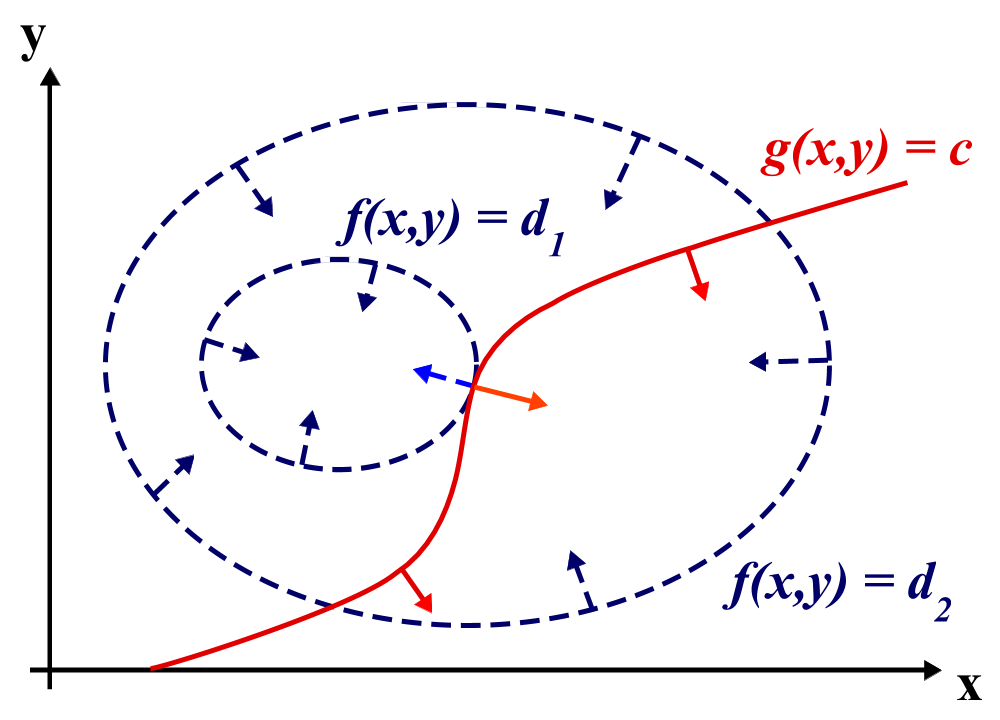
\includegraphics[width=0.5\linewidth]{figs/lagrangian-optimization.png}
\end{center}
If the gradients were not parallel, we could move along $g(x,y)=c$ to a higher contour of $f(x,y)$ by following the component of $\nabla f$ parallel to $g(x,y)=c$.

\newpage
\section{Functional Derivatives}\label{app:functional-optimization}

A functional is just a function of a function -- i.e.\ some rule $F$ that maps a function $f$ into a number $F[f]$.  Definite integrals are probably the most familiar example.
In order to optimize a functional $F$ with respect to its argument $f$, one needs to take a \textit{functional derivative}.\footnote{\url{http://en.wikipedia.org/wiki/Functional_derivative}}
To motivate the definition of a functional derivative, first consider the definition of an ordinary derivative
\begin{align}
	\fd{f(x)}{x}
\equiv
  \lim_{\e\rightarrow0}
	\fr{f(x+\e)-f(x)}{\e}
\end{align}
and note the following identity, which you can verify using
$
  f(x+\e)
=
  f(x)
+
  \dfd{f(x)}{x}
  \e
+
  \mc{O}(\e^2)
$.
\begin{align}\label{eq:scalar-derivative-trick}
  \lim_{\e\rightarrow0}
	\fr{f(x+\e)-f(x)}{\e}
=&\
\left.
	\fr{df(x+\e)}{d\e}
\right|_{\e=0}
\end{align}
For multivariate functions, we have the concept of a \textit{directional derivative}
\begin{align}\label{eq:directional-derivative}
  \bo{y}\cdot
  \pd{f(\bo{x})}{\bo{x}}
=
  \lim_{\e\rightarrow0}
  \fr{f(\bo{x}+\e\bo{y}) - f(\bo{x})}{\e}
\end{align}
which measures the change in $f(\bo{x})$ in the direction $\bo{y}$.
By analogy to equation \ref{eq:scalar-derivative-trick}, the directional derivative can be evaluated as an ordinary scalar derivative with respect to $\e$.
\begin{align}\label{eq:vector-derivative-trick}
  \bo{y}\cdot
  \pd{f(\bo{x})}{\bo{x}}
=
  \left.
  \fd{f(\bo{x} + \e\bo{y})}{\e}
  \right|_{\e=0}
\end{align}
The functional derivative $\dfr{\d F}{\d f}$ is defined by requiring that it satisfy an equation analogous to \ref{eq:directional-derivative}
\begin{align}
  \int_{-\infty}^{\infty}
  dx'\,
  g(x')
  \fr{\d F[f]}{\d f(x')}
\equiv
  \lim_{\e\rightarrow0}
  \fr{F[f+\e g] - F[f]}{\e}
\end{align}
which we might refer to as a \textit{functional directional derivative}, giving the change in $F$ upon displacing its argument along $g$.
Here, the integral takes the role of the dot product in \ref{eq:directional-derivative}.
Using the same trick as in equations \ref{eq:scalar-derivative-trick} and \ref{eq:vector-derivative-trick}, the functional derivative can be expressed as an ordinary scalar derivative.
\begin{align}
\label{eq:functional-derivative-trick}
  \int_{-\infty}^{\infty}
  dx'\,
  g(x')
  \fr{\d F[f]}{\d f(x')}
=
  \left.
  \fd{F[f+\e g]}{\e}
  \right|_{\e=0}
\end{align}
The standard procedure for evaluating the functional derivative is to first evaluate the right-hand side of equation~\ref{eq:functional-derivative-trick} for an arbitrary $g$ and then infer what $\dfr{\d F[f]}{\d f(x)}$ must be by comparing to the left-hand side.
Equivalently, $g(x')$ can be replaced with a Dirac delta $\d(x-x')$ in order arrive at $\dfr{\d F[f]}{\d f(x)}$ directly.

Using equation \ref{eq:functional-derivative-trick} and the Fundamental Lemma of Calculus of Variations (\Cref{app:fundamental-lemma-of-calculus-of-variations}) the stationarity condition for a functional
\begin{align}
  \fr{\d F[f]}{\d f}
\overset{!}{=}
  0
\end{align}
is equivalent to the following condition.
\begin{align}
  \left.
  \fd{F[f+\e g]}{\e}
  \right|_{\e=0}
\overset{!}{=}
  0
&&
  \text{for all $g(x)$}
\end{align}


\newpage
\section{Fundamental Lemma of Calculus of Variations}\label{app:fundamental-lemma-of-calculus-of-variations}
The \textit{Fundamental Lemma of Calculus of Variations}\footnote{\url{http://en.wikipedia.org/wiki/Fundamental_lemma_of_calculus_of_variations}} says that for continuous functions the condition
\begin{align}
	\int_{-\infty}^\infty dx f(x)\eta(x)
=
	0
\sp\text{ for all $\eta(x)$}
\end{align}
holds only when $f(x)=0$ for all $x$.
We can see this by considering the case $\eta(x)=f(x)$.
Since $f(x)^2$ is nonnegative everywhere, its integral is a positive number whenever $f(x)\neq 0$ on a finite range of $x$ values.

\paragraph{Complex functions.}
Consider an analogous situation of two complex functions $f$ and $g$ that satisfy
\begin{align}
\label{eta}
\int_{-\infty}^\infty dx\
	\eta^*(x)f(x)
+\int_{-\infty}^\infty dx\
	\eta(x)g(x)
=
	0
\sp\text{ for all $\eta(x)$.}
\end{align}
We can show that this can only be satisfied if both $f(x)$ and $g(x)$ separately vanish everywhere. Since $\eta(x)$ is arbitrary, this equation must hold for some other function $\gamma(x) = i \eta(x)$.
\begin{align}
\int_{-\infty}^\infty dx\
	\gamma^*(x)f(x)
+\int_{-\infty}^\infty dx\
	\gamma(x)g(x)
&=
	0
\\[1ex]
\int_{-\infty}^\infty dx\
	[i \eta(x) ]^* f(x)
+\int_{-\infty}^\infty dx\
	[i \eta(x)] g(x)
&=
	0
\\[1ex]
   \label{ieta}
    -i 
    \int_{-\infty}^\infty dx\
	\eta^*(x)  f(x)
+ 
    i \int_{-\infty}^\infty dx\
	\eta(x) g(x)
&=
	0
\end{align}
Adding $i$ times equation (\ref{ieta}) to equation (\ref{eta}) yields:
\begin{equation}
\label{eq:condition-on-f}
	\int_{-\infty}^\infty
	dx\ 
	\eta^*(x)f(x)=0
\sp
  \text{ for all $\eta(x)$.}
\end{equation}
Subtracting $i$ times equation (\ref{ieta}) to equation (\ref{eta}) yields:
\begin{equation}
\label{eq:condition-on-g}
	\int_{-\infty}^\infty
	dx\
	\eta(x)g(x)=0
\sp
  \text{ for all $\eta(x)$.}
\end{equation}
Again by the Fundamental Lemma of Calculus of Variations, equations \ref{eq:condition-on-f} and \ref{eq:condition-on-g} are only satisfied when $f(x)=0$ and $g(x)=0$.\footnote{Since we could always choose $\eta(x)=f(x)$ or $\eta(x)=g^*(x)$, giving integrands $|f(x)|^2$ and $|g(x)|^2$ that are nonnegative everywhere.}


\end{document}